
\documentclass[a4paper,12pt,spanish]{article}

\usepackage[utf8]{inputenc}


\usepackage{blindtext}
%\usepackage{microtype}
\usepackage{amsfonts, amsmath, amsthm, amssymb}
%\usepackage{fancyhdr}
%\usepackage{index}
%\usepackage{multicol}    

\usepackage[T1]{fontenc}
\usepackage[utf8]{inputenc}
\usepackage{graphicx}
\usepackage[spanish,es-tabla]{babel}
\usepackage{url}
\usepackage{enumitem}

\usepackage[unicode=true, pdfusetitle,
bookmarks=true,bookmarksnumbered=false,bookmarksopen=false,
breaklinks=true,pdfborder={0 0 1},backref=false,colorlinks=false]
{hyperref}

\usepackage{listings}


\usepackage{siunitx} %para el sistema internacional
\usepackage[export]{adjustbox}
\usepackage{booktabs} 
\usepackage{subcaption}

\usepackage{float}


\newcommand{\address}[1]{
	\par {\raggedright #1
		\vspace{1.4em}
		\noindent\par}
}


\pagenumbering{gobble}
\include{noNumberPage}
\pagenumbering{arabic}
\setcounter{page}{55}

%tutorial de tablas latex: https://manualdelatex.com/tutoriales/tablas

\usepackage{multirow}

% \usepackage[table,xcdraw]{xcolor}


%Inicio del documento (hasta que se cierre con \end{document}
\begin{document}
	
	
	\title{Circuitos lineales RC y RL: comportamiento sinusoidal permanente}
	
	%\author{Adrián Rivero Fernández}
	\date{}
	
	\maketitle
	
	
	
	\begin{abstract} %resumen
		
	En esta práctica estudiaremos las relaciones entre el voltaje y la corriente que circula por un circuito alimentado con una señal sinusoidal.
	
	Mediremos los voltajes en bornes de distintos componentes y sus desfases, para representar el diagrama vectorial de los distintos voltajes.
	
	También trataremos de observar la influencia de la frecuencia en el módulo y en la fase de los voltajes medidos.
		
	\end{abstract}

\section{Introducción}

\subsection*{Circuito RC:}

Utilizamos la solución particular de la ecuación no homogénea
\[V_o \cos \omega t = R_i + \frac{q}{C} \]
hemos prescindido de lo que ocurre al principio de la conexión, los fenómenos transitorios.

Las soluciones particulares de carga y corriente son 
\[q = \frac{V_o C}{\sqrt{(\omega C R)^2 + 1}} \sin (\omega t + \varphi)\]
\[i = \frac{\omega V_o C}{\sqrt{(\omega C R)^2+ 1}}\cos ( \omega t + \varphi ) \]

siendo 
\[ \varphi = \arctan\left(\frac{1}{\omega C R}\right) \]


\subsection*{Circuito RL:}

La solución particular de la ecuación
\[V_o \cos \omega t= R_i + L \frac{di}{dt}\]

es 
\[
i = \frac{V_o}{\sqrt{R^2 + (\omega L)^2}} \cos(\omega t + \varphi ')
\]
siendo 
\[\varphi ' = \arctan\left(\frac{\omega L}{R}\right)\]


\begin{figure}[H]
	\centering
	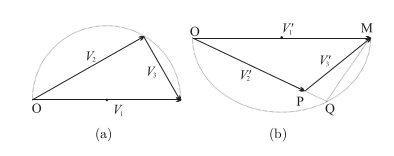
\includegraphics[width=1\linewidth]{diagramas_vectoriales}
	\caption{diagramas vectoriales del circuito RC (a) y el RL (b)}
	\label{fig:diagramasvectoriales}
\end{figure}




\section{Material y métodos}

Utilizaremos un osciloscopio de doble canal, un generador de funciones, un potenciómetro de 10$\si{k\ohm}$, dos condensadores de 0,01 $\si{\micro F}$ y 0,1 $\si{\micro F}$ y dos autoinducciones de 0,3H y 0,15H.

\subsection*{Circuito RC:}

Montamos el circuito de la Figura 2. Utilizamos el osciloscopio en modo X-Y para visualizar la figura de Lissajous. Con eso tomaremos nota del valor de la resistencia y la frecuencia.

Visualizamos en el canal 1 del osciloscopio la caída de tensión, $V_1$ y en el canal 2 visualizamos la caida en la resistencia $V_2$. Medimos también el desfase entre los voltajes.

Después invertimos la señal, con el control de posición vertical del canal 2, y cambiamos el selector de operación de canales a SUMA. Obtenemos $V_3 = V_1 - V_2$.

Repetimos el procedimiento para distintas frecuencias del del generador.


\begin{figure}[H]
	\centering
	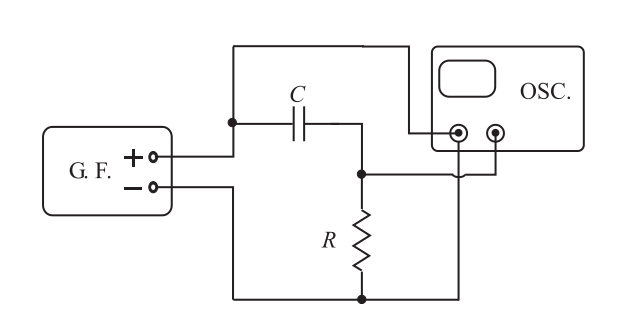
\includegraphics[width=0.8\linewidth]{montaje}
	\caption{montaje}
	\label{fig:montaje}
\end{figure}


\subsection*{Circuito RL:}

Repetimos el mismo procedimiento cambiando el condensador por una autoinducción L en el circuito.


\section{Resultados y discusión}


\subsection*{Circuito RC:}

Los resultados para el condensador 1 y el condensador 2 están anotados, respectivamente, en las Tablas 1 y 2. Las representaciones de los diagramas están en las Figuras 3 y 4.

Para el $\varphi_{teo}$ hemos utilizado:
\[ \varphi_{teo} = \arctan\left(\frac{1}{2\pi f C R}\right) \]


\begin{table}[H]
	\centering
	\begin{tabular}{|lll|lll|}
		\hline
		\multicolumn{3}{|c|}{$C= 0,01 \si{\micro F}$}                                                                 & \multicolumn{3}{c|}{$R = 11030 \si{\ohm}$}                               \\ \hline
		\multicolumn{1}{|l|}{$f$ (kHz)} & \multicolumn{1}{l|}{$\varphi_{teo}$(rad)} & $\varphi_{exp}$ (rad) & \multicolumn{1}{l|}{$V_1 (\si{V})$}  & \multicolumn{1}{l|}{$V_2 (\si{V})$}    & $V_3 (\si{V})$ \\ \hline
		\multicolumn{1}{|l|}{0,1}     & \multicolumn{1}{l|}{1,50}                 & 1,57                     & \multicolumn{1}{l|}{2}   & \multicolumn{1}{l|}{0,125} & 2,004
	     \\ \hline
		\multicolumn{1}{|l|}{0,5}     & \multicolumn{1}{l|}{1,24}                 & 1,13                     & \multicolumn{1}{l|}{2,1} & \multicolumn{1}{l|}{0,7}   & 1,910       \\ \hline
		\multicolumn{1}{|l|}{1}       & \multicolumn{1}{l|}{0,96}                 & 0,94                     & \multicolumn{1}{l|}{2,1} & \multicolumn{1}{l|}{1,2}   & 1,700       \\ \hline
		\multicolumn{1}{|l|}{5}       & \multicolumn{1}{l|}{0,28}                 & 0,29                     & \multicolumn{1}{l|}{2,1} & \multicolumn{1}{l|}{2}     & 0,600       \\ \hline
		\multicolumn{1}{|l|}{10}      & \multicolumn{1}{l|}{0,14}                 & 0,14                     & \multicolumn{1}{l|}{2,1} & \multicolumn{1}{l|}{2,05}  & 0,301      \\ \hline
		\multicolumn{1}{|l|}{15}      & \multicolumn{1}{l|}{0,10}                 & 0,10                     & \multicolumn{1}{l|}{2,1} & \multicolumn{1}{l|}{2,1}   & 0,200         \\ \hline
	\end{tabular}
	\caption{Resultados para el condensador 1}
	\label{tab:my-table}
\end{table}


\begin{figure}[H]
	\centering
	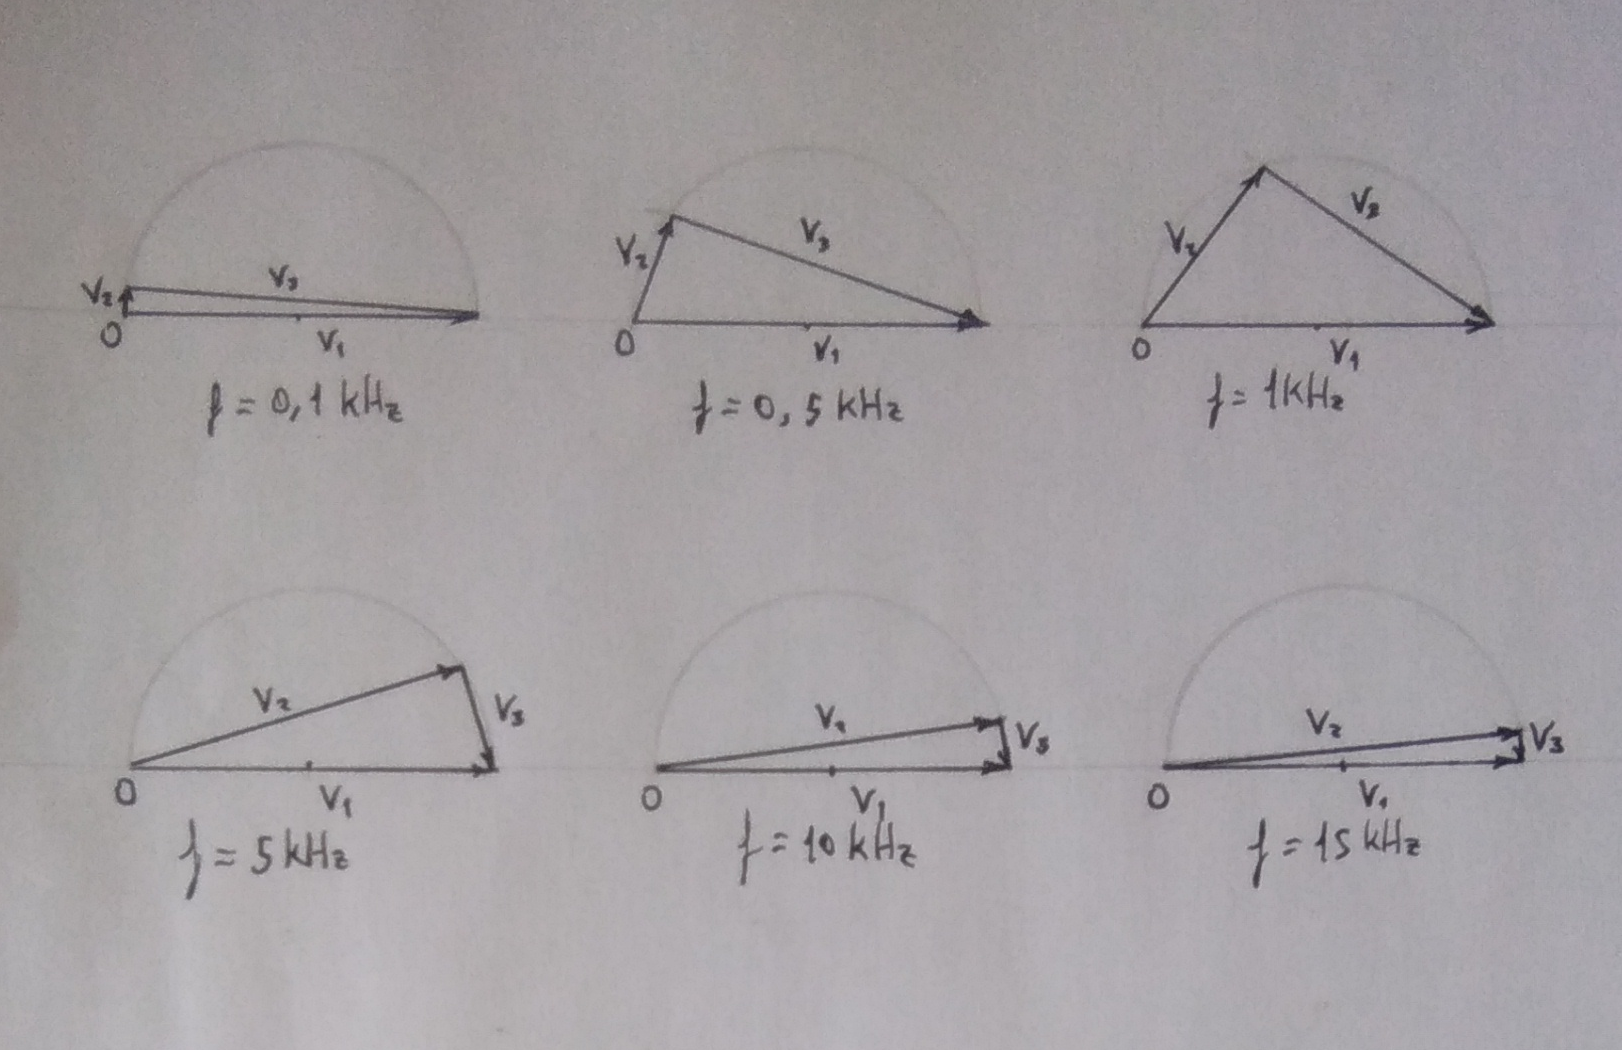
\includegraphics[width=0.8\linewidth]{../diagramas/RC1}
	\caption{Diagramas para el condensador 1}
	\label{fig:montaje}
\end{figure}



\begin{table}[H]
	\centering
	\begin{tabular}{|lll|lll|}
		\hline
		\multicolumn{3}{|c|}{$C= 0,1 \si{\micro F}$}                                                                  & \multicolumn{3}{c|}{$R = 1016 \si{\ohm}$}                                \\ \hline
		\multicolumn{1}{|l|}{$f$ (kHz)} & \multicolumn{1}{l|}{$\varphi_{teo}$(rad)} & $\varphi_{exp}$ (rad) & \multicolumn{1}{l|}{$V_1 (\si{V})$}  & \multicolumn{1}{l|}{$V_2 (\si{V})$}    & $V_3 (\si{V})$ \\ \hline
		\multicolumn{1}{|l|}{0,1}     & \multicolumn{1}{l|}{1,51}                 & 1,57                     & \multicolumn{1}{l|}{2,1}  & \multicolumn{1}{l|}{0,2}  & 2,109       \\ \hline
		\multicolumn{1}{|l|}{0,5}     & \multicolumn{1}{l|}{1,26}                 & 1,13                     & \multicolumn{1}{l|}{2,1}  & \multicolumn{1}{l|}{0,7}  & 1,910       \\ \hline
		\multicolumn{1}{|l|}{1}       & \multicolumn{1}{l|}{1,00}                 & 0,94                     & \multicolumn{1}{l|}{2,1}  & \multicolumn{1}{l|}{1}    & 1,716       \\ \hline
		\multicolumn{1}{|l|}{5}       & \multicolumn{1}{l|}{0,30}                 & 0,34                     & \multicolumn{1}{l|}{2,1}  & \multicolumn{1}{l|}{1,9}  & 0,705       \\ \hline
		\multicolumn{1}{|l|}{10}      & \multicolumn{1}{l|}{0,16}                 & 0,17                     & \multicolumn{1}{l|}{2,1}  & \multicolumn{1}{l|}{2}    & 0,357       \\ \hline
		\multicolumn{1}{|l|}{15}      & \multicolumn{1}{l|}{0,10}                 & 0,10                     & \multicolumn{1}{l|}{2,05} & \multicolumn{1}{l|}{2,05} & 0,200         \\ \hline
	\end{tabular}
	\caption{Resultados para el condensador 2}
	\label{tab:my-table}
\end{table}

\begin{figure}[H]
	\centering
	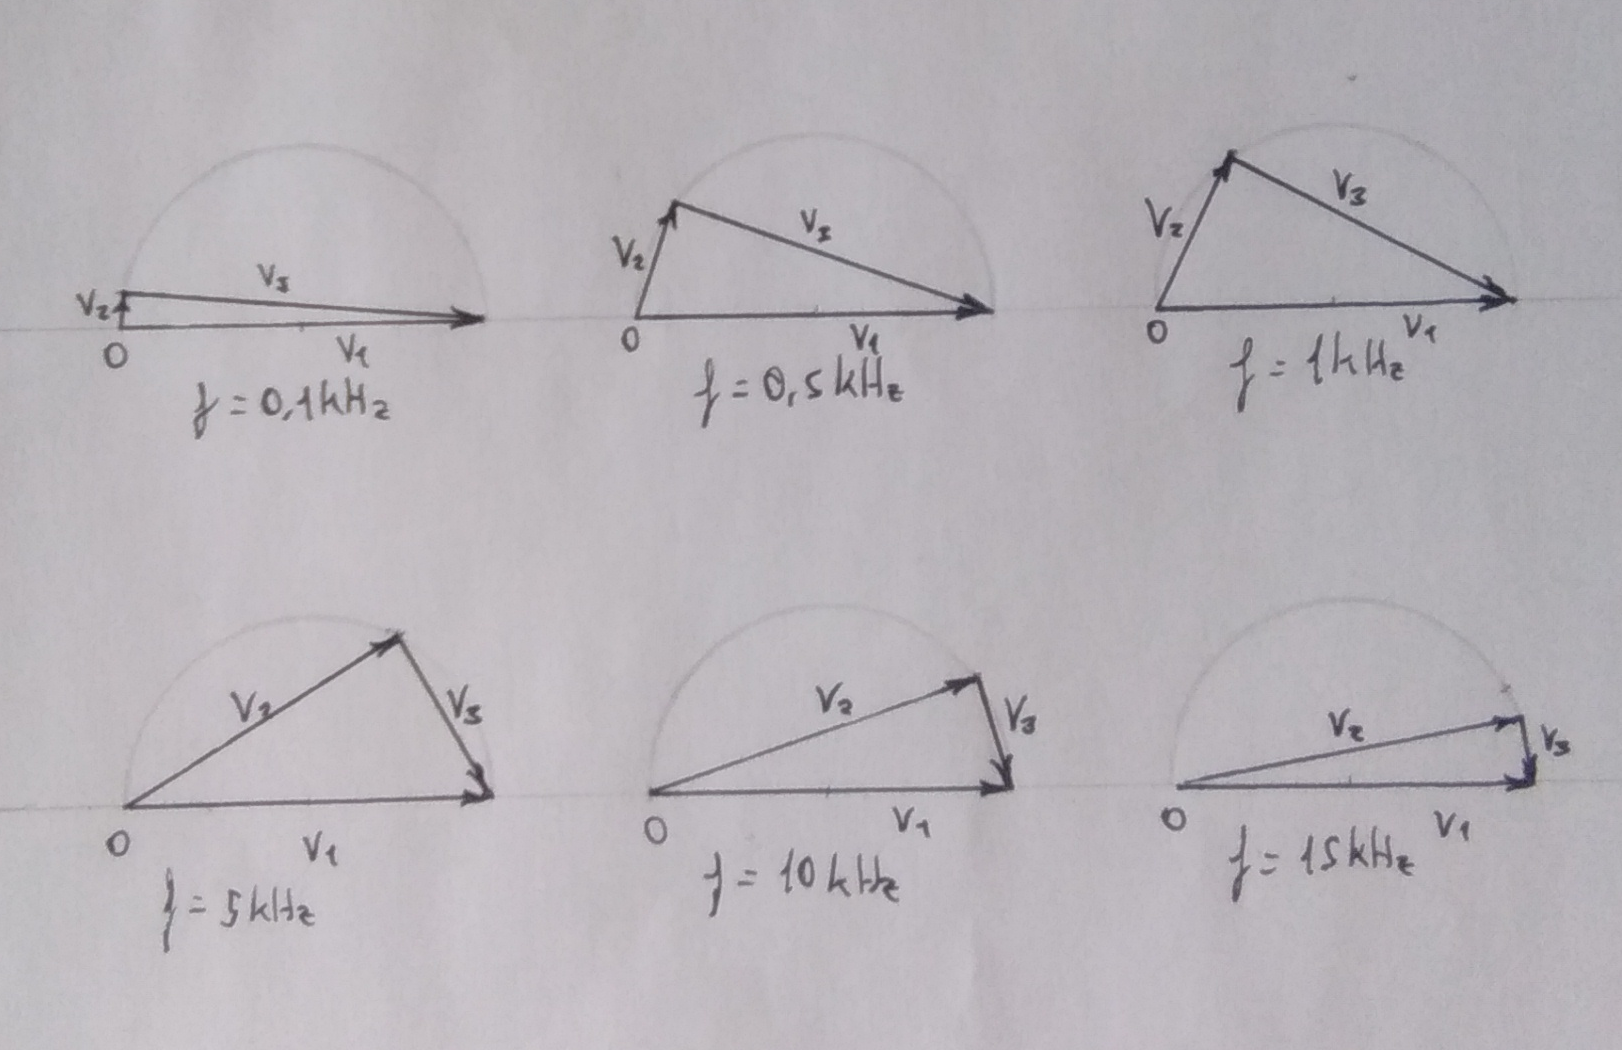
\includegraphics[width=0.8\linewidth]{../diagramas/RC2}
	\caption{Diagramas para el condensador 2}
	\label{fig:montaje}
\end{figure}



\subsection*{Circuito RL:}

Los resultados para la bobina 1 y la bobina 2 están anotados, respectivamente, en las Tablas 3 y 4.
Las representaciones de los diagramas están en las Figuras 5 y 6.

Para el $\varphi_{teo}$ hemos utilizado:
\[ \varphi_{teo} = \arctan\left(\frac{2\pi f L}{R}\right) \]


\begin{table}[H]
	\centering
	\begin{tabular}{|lll|lll|}
		\hline
		\multicolumn{3}{|c|}{L= 0,3 H}                                                                       & \multicolumn{3}{c|}{$R = 11030 \si{\ohm}$}                              \\ \hline
		\multicolumn{1}{|l|}{$f$ (kHz)} & \multicolumn{1}{l|}{$\varphi_{teo}$(rad)} & $\varphi_{exp}$ (rad) & \multicolumn{1}{l|}{$V_1 (\si{V})$}  & \multicolumn{1}{l|}{$V_2 (\si{V})$}    & $V_3 (\si{V})$ \\ \hline
		\multicolumn{1}{|l|}{0,1}     & \multicolumn{1}{l|}{0,02}                 & 0,10                     & \multicolumn{1}{l|}{2,1} & \multicolumn{1}{l|}{2,1} & 0,200         \\ \hline
		\multicolumn{1}{|l|}{0,5}     & \multicolumn{1}{l|}{0,09}                 & 0,12                     & \multicolumn{1}{l|}{2,1} & \multicolumn{1}{l|}{2,1} & 0,250         \\ \hline
		\multicolumn{1}{|l|}{1}       & \multicolumn{1}{l|}{0,17}                 & 0,17                     & \multicolumn{1}{l|}{2,1} & \multicolumn{1}{l|}{2,1} & 0,351         \\ \hline
		\multicolumn{1}{|l|}{5}       & \multicolumn{1}{l|}{0,71}                 & 0,73                     & \multicolumn{1}{l|}{2,1} & \multicolumn{1}{l|}{1,6} & 1,400       \\ \hline
		\multicolumn{1}{|l|}{10}      & \multicolumn{1}{l|}{1,04}                 & 1,03                     & \multicolumn{1}{l|}{2,1} & \multicolumn{1}{l|}{0,9} & 1,809       \\ \hline
		\multicolumn{1}{|l|}{15}      & \multicolumn{1}{l|}{1,20}                 & 1,57                     & \multicolumn{1}{l|}{2,1} & \multicolumn{1}{l|}{0,7} & 2,214       \\ \hline
	\end{tabular}
	\caption{Resultados para la bobina 1}
	\label{tab:my-table}
\end{table}

\begin{figure}[H]
	\centering
	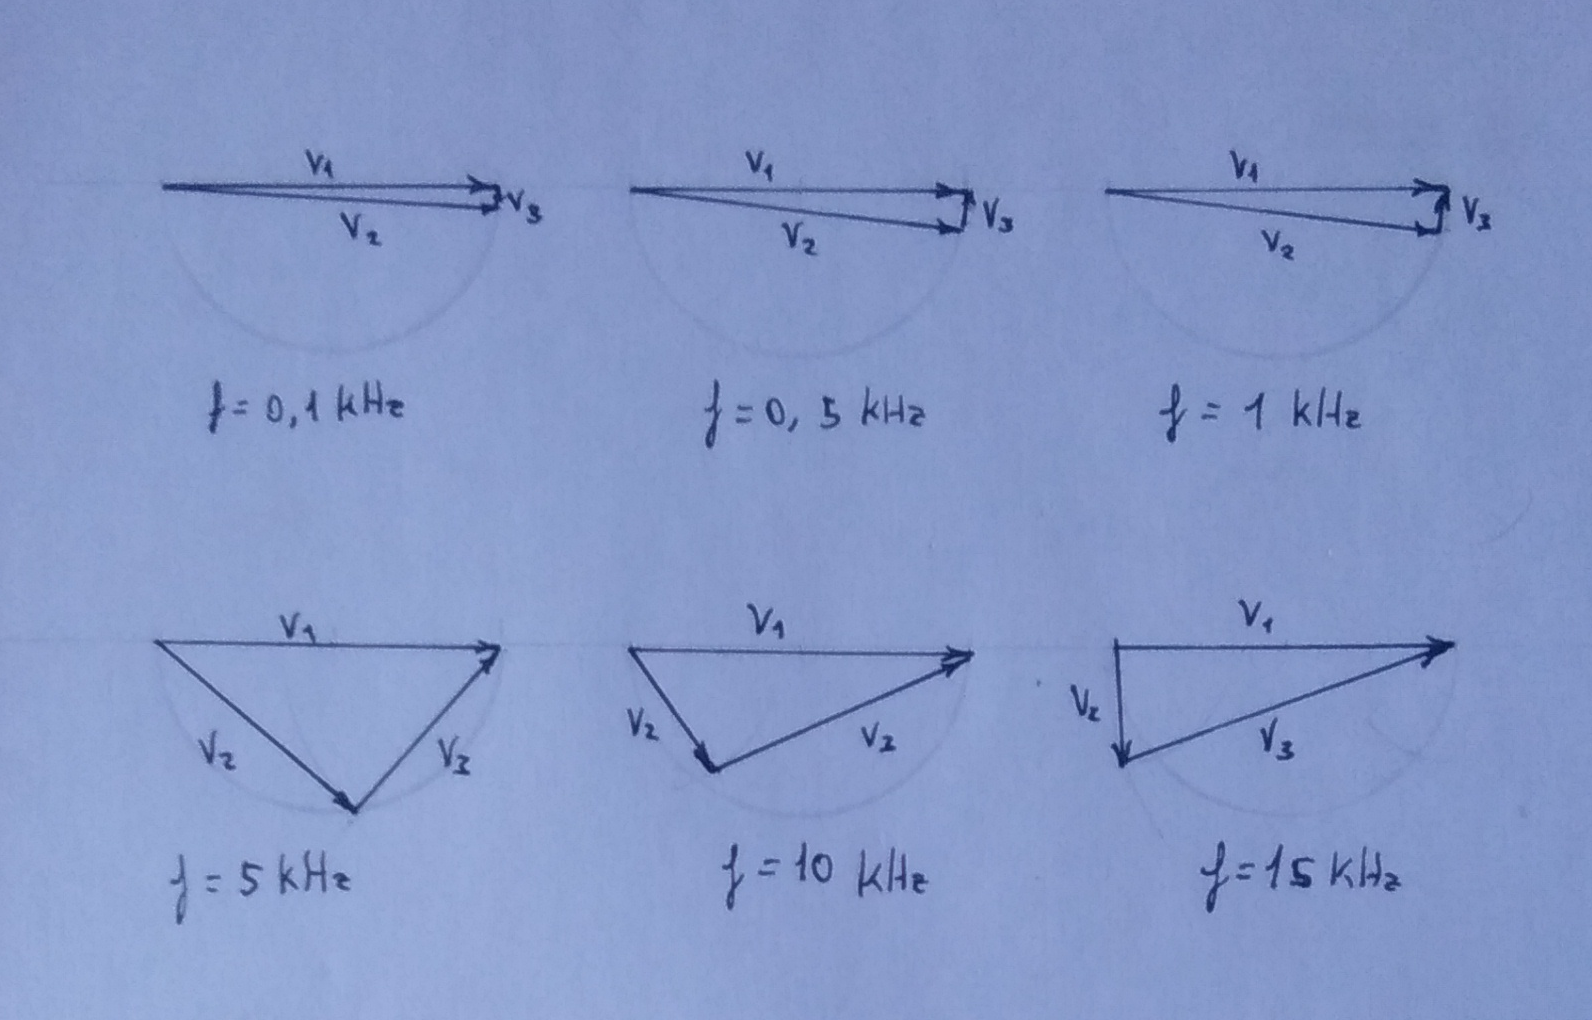
\includegraphics[width=0.8\linewidth]{../diagramas/LC1}
	\caption{Diagramas para la bobina 1}
	\label{fig:montaje}
\end{figure}



\begin{table}[H]
	\centering
	\begin{tabular}{|lll|lll|}
		\hline
		\multicolumn{3}{|c|}{L= 0,15 H}                                                                      & \multicolumn{3}{c|}{R = 1016 $\Omega$}                                \\ \hline
		\multicolumn{1}{|l|}{$f$ (kHz)} & \multicolumn{1}{l|}{$\varphi_{teo}$(rad)} & $\varphi_{exp}$ (rad) & \multicolumn{1}{l|}{$V_1 (\si{V})$}  & \multicolumn{1}{l|}{$V_2 (\si{V})$}    & $V_3 (\si{V})$ \\ \hline
		\multicolumn{1}{|l|}{0,1}     & \multicolumn{1}{l|}{0,09}                 & 0,12                     & \multicolumn{1}{l|}{2,1}  & \multicolumn{1}{l|}{1,9} & 0,311       \\ \hline
		\multicolumn{1}{|l|}{0,5}     & \multicolumn{1}{l|}{0,43}                 & 0,31                     & \multicolumn{1}{l|}{2,1}  & \multicolumn{1}{l|}{1,8} & 0,679       \\ \hline
		\multicolumn{1}{|l|}{1}       & \multicolumn{1}{l|}{0,75}                 & 0,52                     & \multicolumn{1}{l|}{2,1}  & \multicolumn{1}{l|}{1,6} & 1,073       \\ \hline
		\multicolumn{1}{|l|}{5}       & \multicolumn{1}{l|}{1,36}                 & 1,13                     & \multicolumn{1}{l|}{2,1}  & \multicolumn{1}{l|}{0,7} & 1,910       \\ \hline
		\multicolumn{1}{|l|}{10}      & \multicolumn{1}{l|}{1,46}                 & 1,35                     & \multicolumn{1}{l|}{2,05} & \multicolumn{1}{l|}{0,3} & 2,006      \\ \hline
		\multicolumn{1}{|l|}{15}      & \multicolumn{1}{l|}{1,50}                 & 1,57                     & \multicolumn{1}{l|}{2,05} & \multicolumn{1}{l|}{0,2} & 2,060      \\ \hline
	\end{tabular}
	\caption{Resultados para la bobina 2}
	\label{tab:my-table}
\end{table}

\begin{figure}[H]
	\centering
	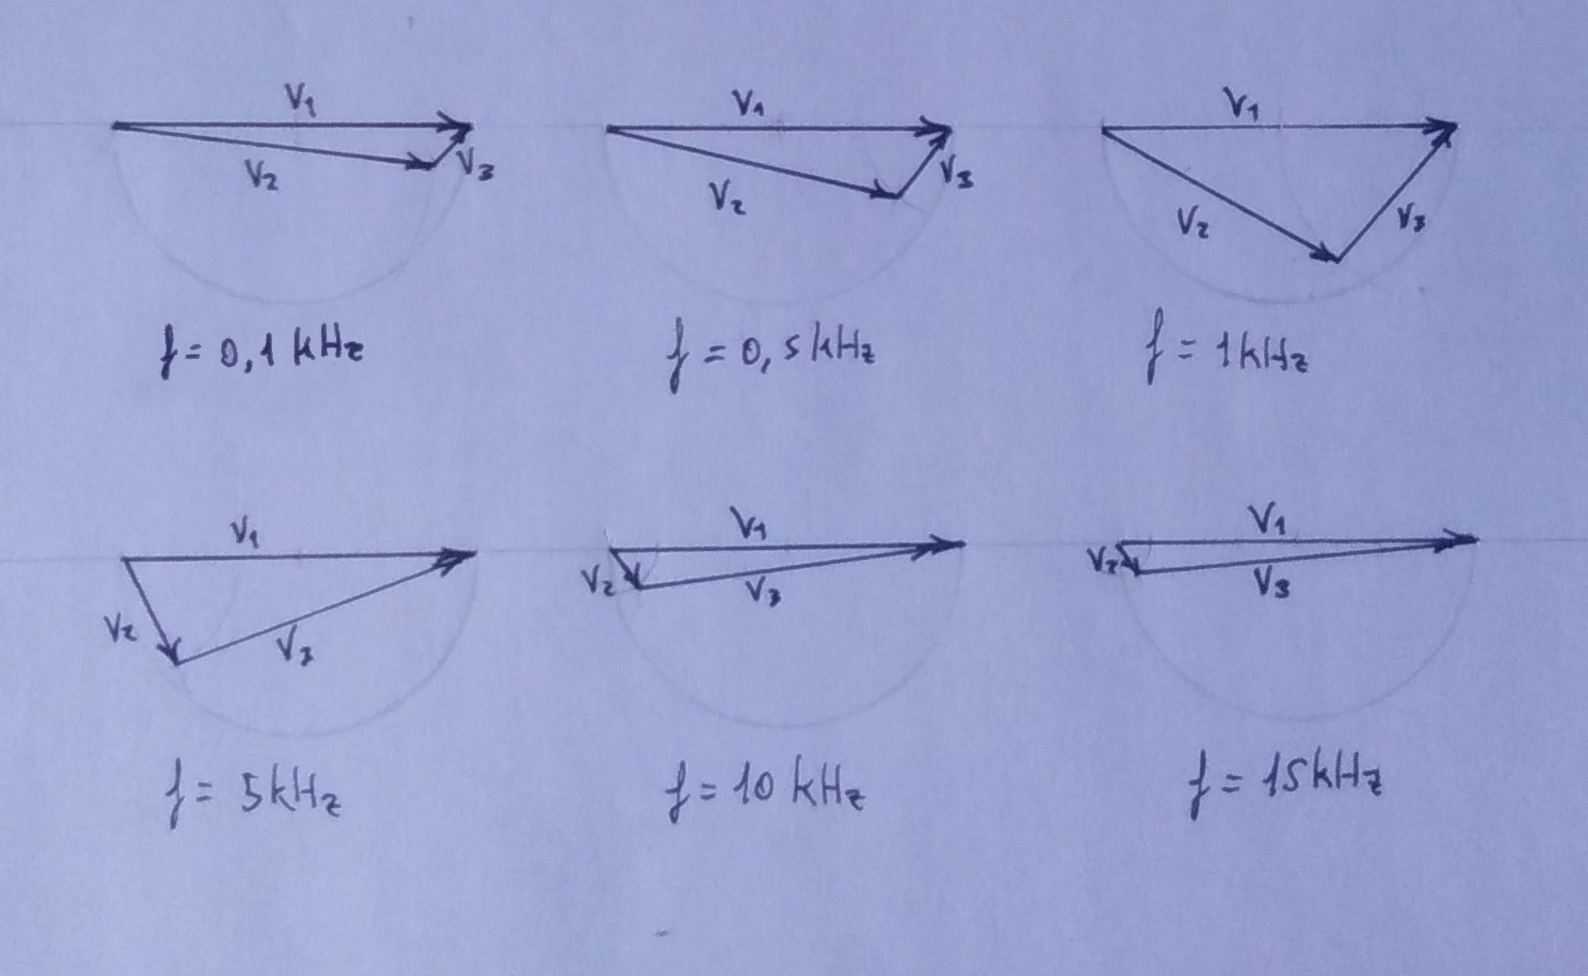
\includegraphics[width=0.8\linewidth]{../diagramas/LC2}
	\caption{Diagramas para la bobina 2}
	\label{fig:montaje}
\end{figure}









%%%%%%%%%%%%%%%%%%%%%%%%%%%
\begin{thebibliography}{3}
	%%%%%%%%%%%%%%%%%%%%%%%%%%%
	
	
	\bibitem{UNED2022} (varios) Guiones de prácticas- Técnicas Experimentales II. Grado en Física. Versión 2.1  UNED, 2022 \url{https://2022.cursosvirtuales.uned.es/o/3754218}
	%	\bibitem{UNED2021} (varios) Técnicas Experimentales I. Versión 3.5.  UNED, 2021 \url{https://2021.cursosvirtuales.uned.es/o/42035617}
	%\bibitem{2021} Densidad de materiales \url{ https://www.stemm.com/index.php/es/densidades-de-materiales }
	
	
\end{thebibliography}


\end{document}



